\subsection{Xác thực và phân quyền — JWT hai tầng}

\subsubsection{Kiến trúc cặp token tách biệt}

Hệ thống sử dụng \textbf{hai khóa bí mật JWT riêng biệt} cho hai loại token khác nhau: \texttt{JWT\_ACCESS\_SECRET} dùng để ký và xác thực \textit{access token}, còn \texttt{JWT\_REFRESH\_SECRET} chỉ tồn tại trong dịch vụ Identity và dùng để ký \textit{refresh token}. Việc tách biệt này đảm bảo lộ một secret không kéo theo lộ secret còn lại; đồng thời BFF chỉ cần giữ \texttt{JWT\_ACCESS\_SECRET} để xác thực cục bộ mà không có khả năng tự cấp refresh token mới.

\begin{table}[H]
\centering
\caption{So sánh access token và refresh token}
\label{tab:so-sanh-jwt}
\begin{tabularx}{\textwidth}{|L{0.2}|L{0.2}|L{0.3}|L{0.3}|}
\hline
\textbf{Loại token} & \textbf{Thời hạn} & \textbf{Lưu tại} & \textbf{Mục đích sử dụng} \\
\hline
\texttt{accessToken} & 15 phút & Bộ nhớ trình duyệt cử tri & Đính kèm mọi yêu cầu API \\
\hline
\texttt{refreshToken} & 7 ngày & Redis (\texttt{refreshToken:\{userId\}}) & Cấp cặp token mới khi hết hạn \\
\hline
\end{tabularx}
\end{table}

Phần dữ liệu (\textit{payload}) của JWT chứa các trường tối thiểu cần thiết cho phân quyền: định danh người dùng \texttt{sub}, địa chỉ thư điện tử, vai trò (\texttt{ADMIN}, \texttt{VOTER} hoặc \texttt{CANDIDATE}) và cờ \texttt{isActive}. Không có dữ liệu nhạy cảm nào được nhúng vào payload vì JWT không được mã hóa — chỉ được ký.

\subsubsection{Xoay vòng refresh token}

Mỗi lần làm mới phiên, hệ thống thực hiện \textbf{xoay vòng hoàn toàn} (\textit{rotation}): xóa refresh token cũ khỏi Redis rồi cấp một cặp \texttt{accessToken}/\texttt{refreshToken} mới. Cơ chế này phát hiện ngay tấn công \textit{refresh token reuse} — kẻ tấn công chiếm được refresh token cũ sẽ thấy entry trong Redis đã bị xóa, do đó buộc phải đăng nhập lại bằng mật khẩu. Hàm \texttt{rotateRefreshToken} của dịch vụ Identity được trình bày trong Hình~\ref{fig:token-rotation}.

\begin{figure}[H]
    \centering
    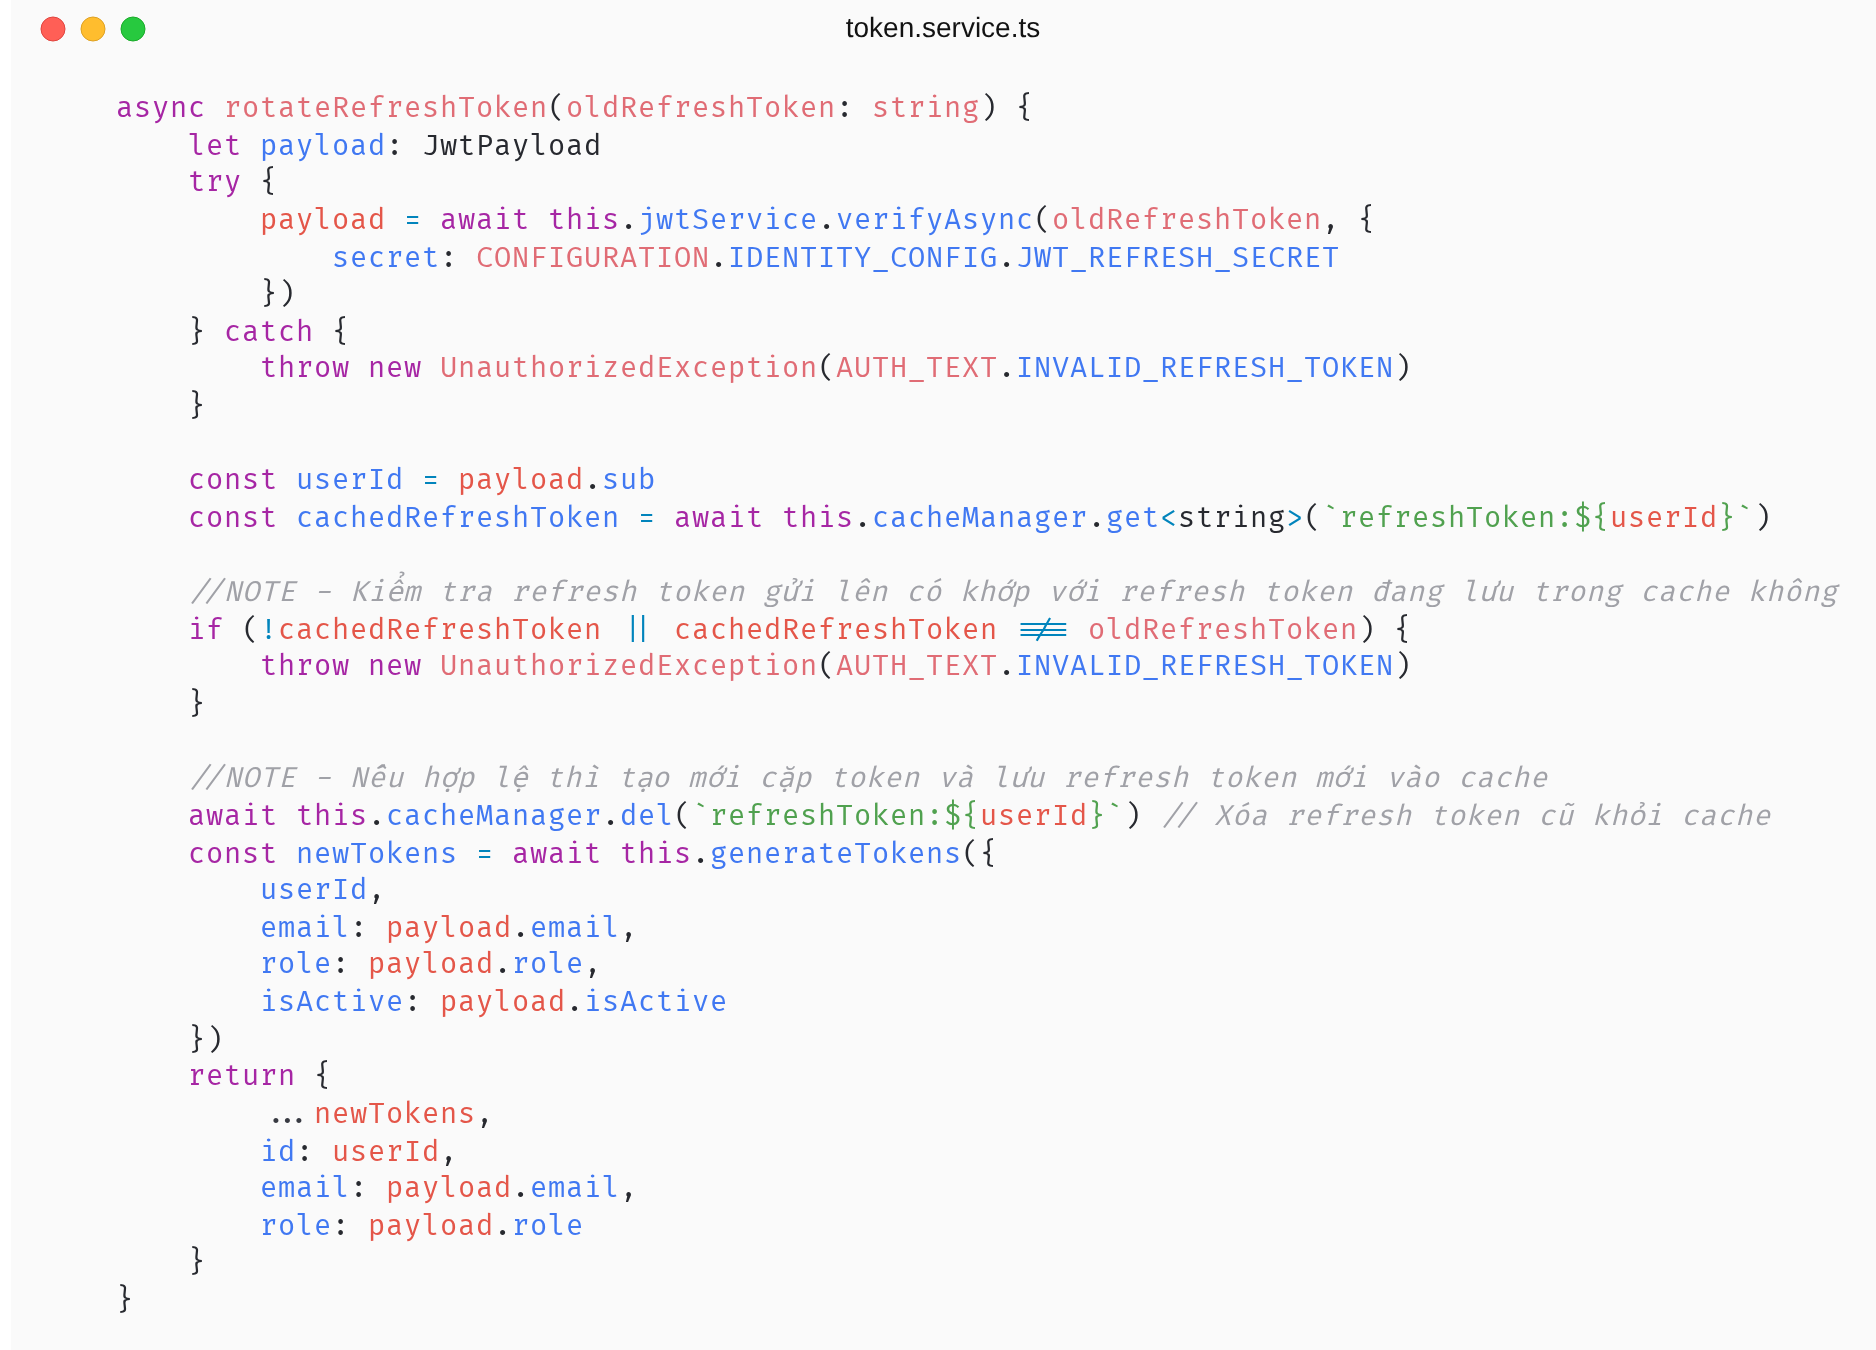
\includegraphics[width=0.85\textwidth, keepaspectratio]{Figures/code/token-rotation.png}
    \caption{Hàm \texttt{rotateRefreshToken} thực hiện xoay vòng refresh token tại Identity}
    \label{fig:token-rotation}
\end{figure}

Quy trình bên trong gồm bốn bước tuần tự: (1) xác thực chữ ký refresh token bằng \texttt{JWT\_REFRESH\_SECRET}; (2) đối chiếu giá trị token người dùng gửi lên với giá trị đang lưu tại Redis — nếu khác nhau hoặc không tồn tại thì từ chối; (3) xóa entry Redis cũ; (4) sinh cặp token mới và ghi đè entry Redis. Bốn bước này được thực hiện đồng bộ trong một hàm để tránh khoảng cửa sổ tấn công giữa các bước.

\subsubsection{Xác thực cục bộ tại BFF — bỏ qua vòng gọi lại Identity}

BFF xác thực \texttt{accessToken} \textbf{cục bộ} bằng \texttt{JWT\_ACCESS\_SECRET} mà không cần gọi sang Identity service. Tiếp cận này loại bỏ một vòng gọi TCP cho mỗi yêu cầu — giảm độ trễ trung bình từ 5 đến 15 ms và tránh tải dồn lên dịch vụ Identity vốn phục vụ cả các thao tác đăng nhập, đăng ký, quản trị tài khoản. Quy trình kiểm tra trong \texttt{AuthenticatorGuard} được trình bày trong Hình~\ref{fig:auth-guard-jwt-verify}.

\begin{figure}[H]
    \centering
    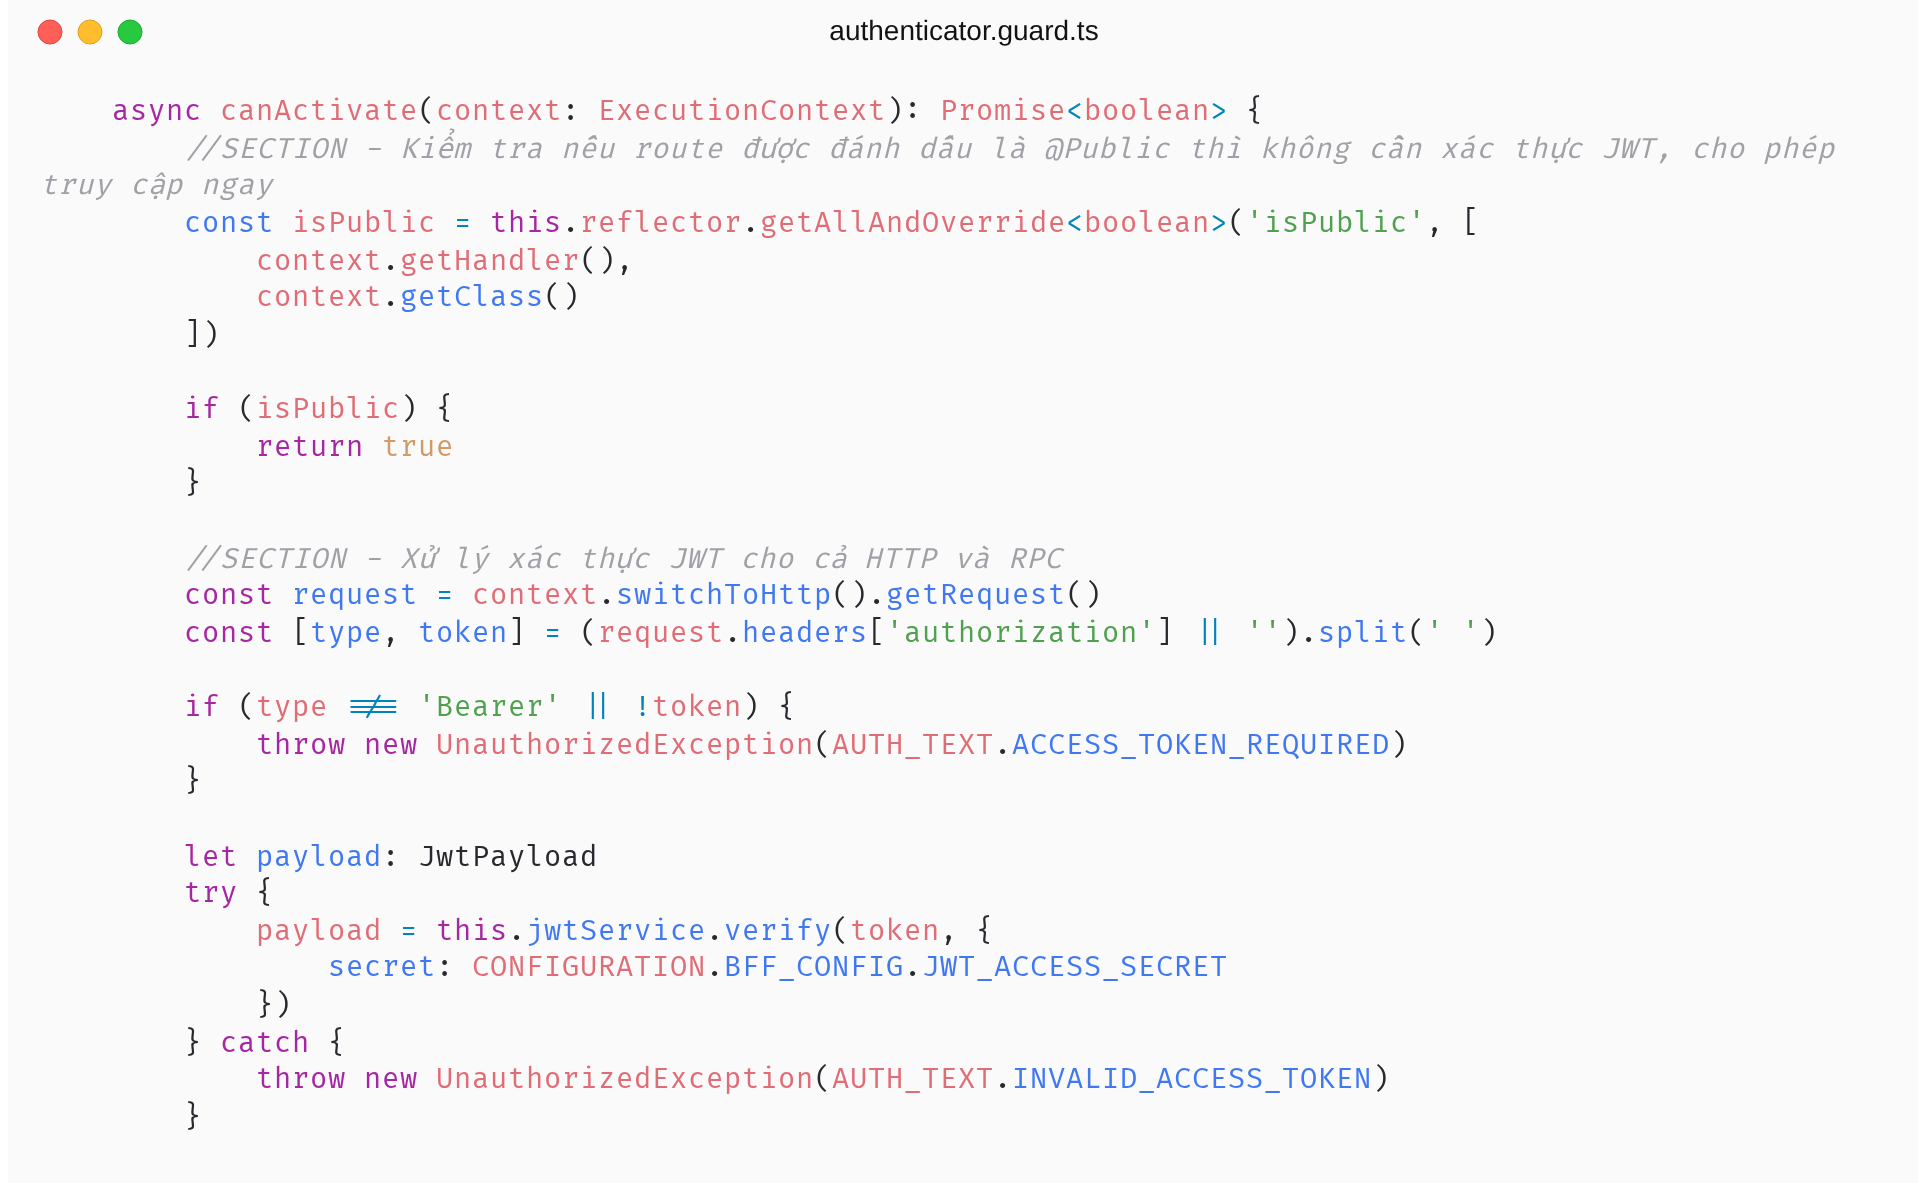
\includegraphics[width=0.85\textwidth, keepaspectratio]{Figures/code/auth-guard-jwt-verify.png}
    \caption{Lớp \texttt{AuthenticatorGuard} của BFF xác thực JWT cục bộ}
    \label{fig:auth-guard-jwt-verify}
\end{figure}

Sau khi xác thực thành công, payload được gắn vào đối tượng \texttt{request} dưới khóa \texttt{user} để các tầng tiếp theo (controller, service) dùng được mà không phải giải mã lại. Cơ chế \textit{blacklist} bằng Redis cho phép vô hiệu hóa ngay lập tức một tài khoản đang hoạt động (ví dụ khi quản trị viên khóa cử tri vi phạm) mà không phải chờ access token hết hạn 15 phút.

\subsubsection{Kiểm soát truy cập theo vai trò}

Phân quyền được thực hiện qua decorator \texttt{@Roles(\textquotesingle ADMIN\textquotesingle)} đặt trên controller hoặc route handler. Lớp \texttt{RolesGuard} đọc metadata này thông qua \texttt{Reflector} của NestJS, so sánh với \texttt{payload.role} và từ chối yêu cầu nếu không trùng. Decorator \texttt{@Public()} đánh dấu các route không yêu cầu xác thực — chủ yếu là các endpoint công khai phục vụ kiểm chứng phiếu bầu hoặc xem kết quả sau khi cuộc bầu cử kết thúc.

Bên cạnh kiểm soát theo vai trò, BFF còn kiểm tra tiêu đề \texttt{Origin} của yêu cầu đăng nhập: nếu một tài khoản có vai trò \textit{VOTER} hoặc \textit{CANDIDATE} đăng nhập vào trang quản trị (Admin Web), hệ thống trả về lỗi \texttt{401 Unauthorized}. Cơ chế này ngăn cử tri vô tình hoặc cố ý xâm nhập giao diện quản trị — tách bạch hoàn toàn hai miền sử dụng dù chia sẻ cùng một dịch vụ Identity.
